% %%%%%%%%%%%%%%%%%%%%%%%%%%%%%%%%%%%%%%%%%%%%%%%%%%%%%%%%%%%%%%%%%%%%%%
% Dummy Chapter:
% %%%%%%%%%%%%%%%%%%%%%%%%%%%%%%%%%%%%%%%%%%%%%%%%%%%%%%%%%%%%%%%%%%%%%%

% %%%%%%%%%%%%%%%%%%%%%%%%%%%%%%%%%%%%%%%%%%%%%%%%%%%%%%%%%%%%%%%%%%%%%%
% The Introduction:
% %%%%%%%%%%%%%%%%%%%%%%%%%%%%%%%%%%%%%%%%%%%%%%%%%%%%%%%%%%%%%%%%%%%%%%
\fancychapter{Implementation}
\label{cap:implement}


In this chapter, a detailed explanation of the implemented system will be provided. Figure \ref{fig:implementation} provides an expanded view of the already presented Figure \ref{fig:solution}. In order to implement the system, several decisions were made. Starting with the beacon, the chosen technology was \ac{BLE}, leading to the usage of \ac{BLE}-enabled beacons. This decision is fundamental for defining the software that is to be use for smartphone-beacon communication, in this case being the \ac{BLE} stack. For the map server, the Google maps service was   
used, and as such the map service component of the smartphone was implemented through the Google maps API. The algorithm implemented on the location server was a Cell of Origin (CoO), which was described on Section \ref{sec:techniques}, that made use of beacon information stored onto a database, for calculating positions. This database is represented by the beacon manager component of the location server. 

\begin{figure}[H]
	\centering
		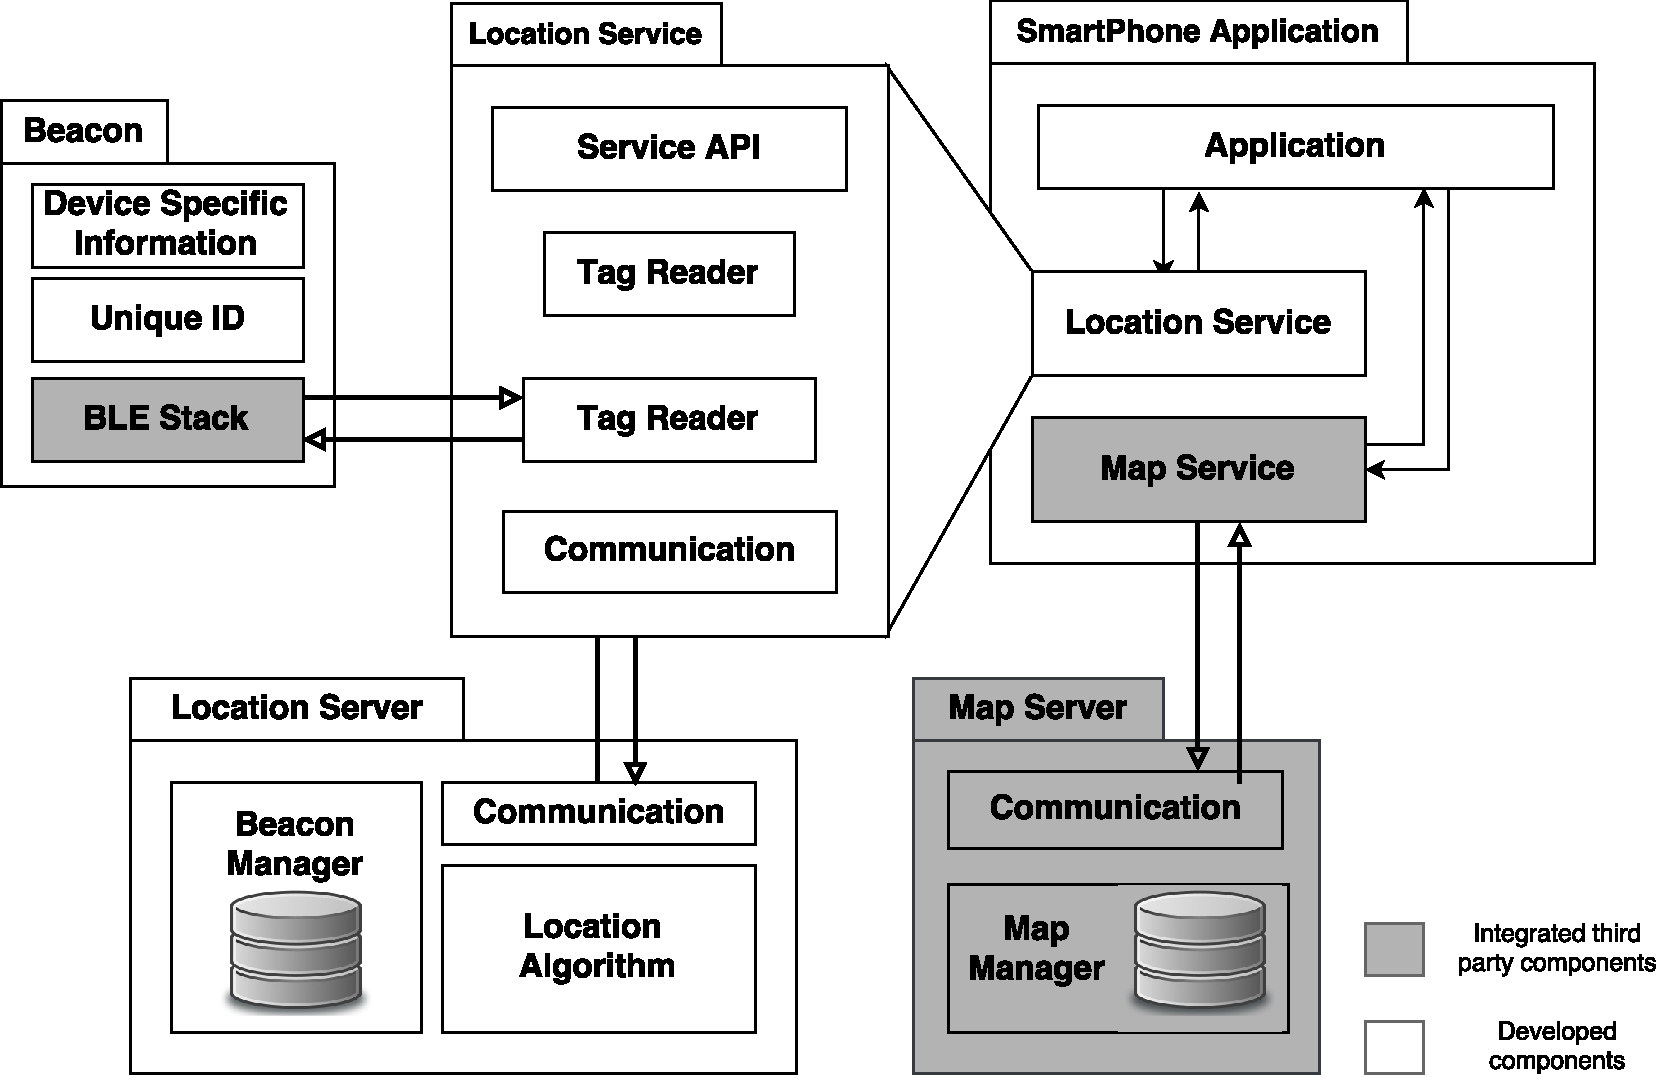
\includegraphics[width=1\linewidth]{4.Chapter/detailedArch.pdf}
	\caption[Detailed system Architecture]{Detailed system Architecture}
	\label{fig:implementation}
\end{figure}

\section{Location algorithm} 
\label{sec:algos} 
 
 
The location algorithm is in charge of calculating a position from a set of data that it has received. This data is dependent on the beacons and is formed by a group of pairs of data. Each pair is composed by one of the metrics presented in section \ref{sec:techniques} and the ID of the beacon associated to it. As such the data that is given to the algorithm is a list of pairs that was collected by the location server. 
 
 
The deployed algorithm can be of different types, depending on the demanded system's location precision. In this implementation, the chosen algorithm was a Cell of Origion (CoO). This implementation choice allowed for a less complex implementation of the location server, while still being capable of calculating locations. The location algorithm starts by confirming that all the received beacons are present in its database. Having confirmed that, it analyses the list in search for the highest metric value. The user's location is presumed to be equal to the location of the beacon with the highest metric. 
 
\section{ Beacons}  
\label{sec:beacon}  
  
  
\subsection{Communication protocol}  
\label{sec:commprot}  
  
  
The used technology on the beacons was Bluetooth low energy, which has already been introduced on Section \ref{sec:indoortech}. For better understanding the beacon-smartphone communication, it is fundamental to comprehend how this technology works. All the presented information on \ac{BLE} was obtained from its core manual \cite{BLECore}.  
  
 
 
The smartphone and the beacon are set up as two complementary classes. The beacon is defined as a peripheral, a role used to describe devices optimized to support a single connection. This role allows it to have a reduced complexity, since it's only required to function as a slave, an entity that is only capable of receiving connections. On the other hand, the smartphone is defined by the complementary role, central. A central device is capable of supporting multiple connections and is responsible for initiating all of them.  
  
  
 
 
  
  
Another important aspect in understanding this technology is the \ac{BLE} profiles. A profile, which can be seen on Figure \ref{fig:profile} defines an hierarchy in which a device's available services are organized. By doing so, a system's profile ends up defining the applications behaviour and data formats, as well as the manner in which data is exchanged. The hierarchy is composed by two parts: Services and Characteristics.  
  
  
\begin{itemize}  
  
  
\item A profile is composed by one or more services. A service is a collection of data and associated behaviours to accomplish a particular function or feature of a device or portions of a device. It can be either primary, which provides primary functionalities of a device, or secondary, providing auxiliary functionalities of a device and being referenced from at least one primary service. A service is composed of characteristics and/or references to other services.  
  
  
\item A Characteristic is a value that is used in a service that has properties and configuration information that describe how the value should be accessed as well as information on how to display the value. A characteristic is defined by its declaration, its properties, its value and may also be defined by its descriptor, which describes the value or permit configuration of  
the server relative to the value.  
\end{itemize}  
  
\begin{figure}[H]  
\centering  
\includegraphics[width=0.5\linewidth]{2.Chapter/profile.png}  
\caption[Gatt-based profile hierarchy]{Gatt-based profile hierarchy}  
\label{fig:profile}  
\end{figure}  
 
 
  
\subsection{\ac{BLE} enable beacons}  
\label{sec:ble-beacon}  
 
 
 
 
The used beacons are Texas Instruments CC2650STK devices which can be visualised in Figure ~\ref{fig:beacon}. Alongside the device, which comes with a pre-installed Bluetooth low energy program capable of giving information on each of its ten sensors through its predefined profiles, there is a texas smartphone application that can connect to a single device and read from its sensors. By using the texas Code Composer Studio (CSS), the predefined \ac{BLE} profile existent on the device could be changed.  
 
 
 \begin{figure} [H] 
\centering  
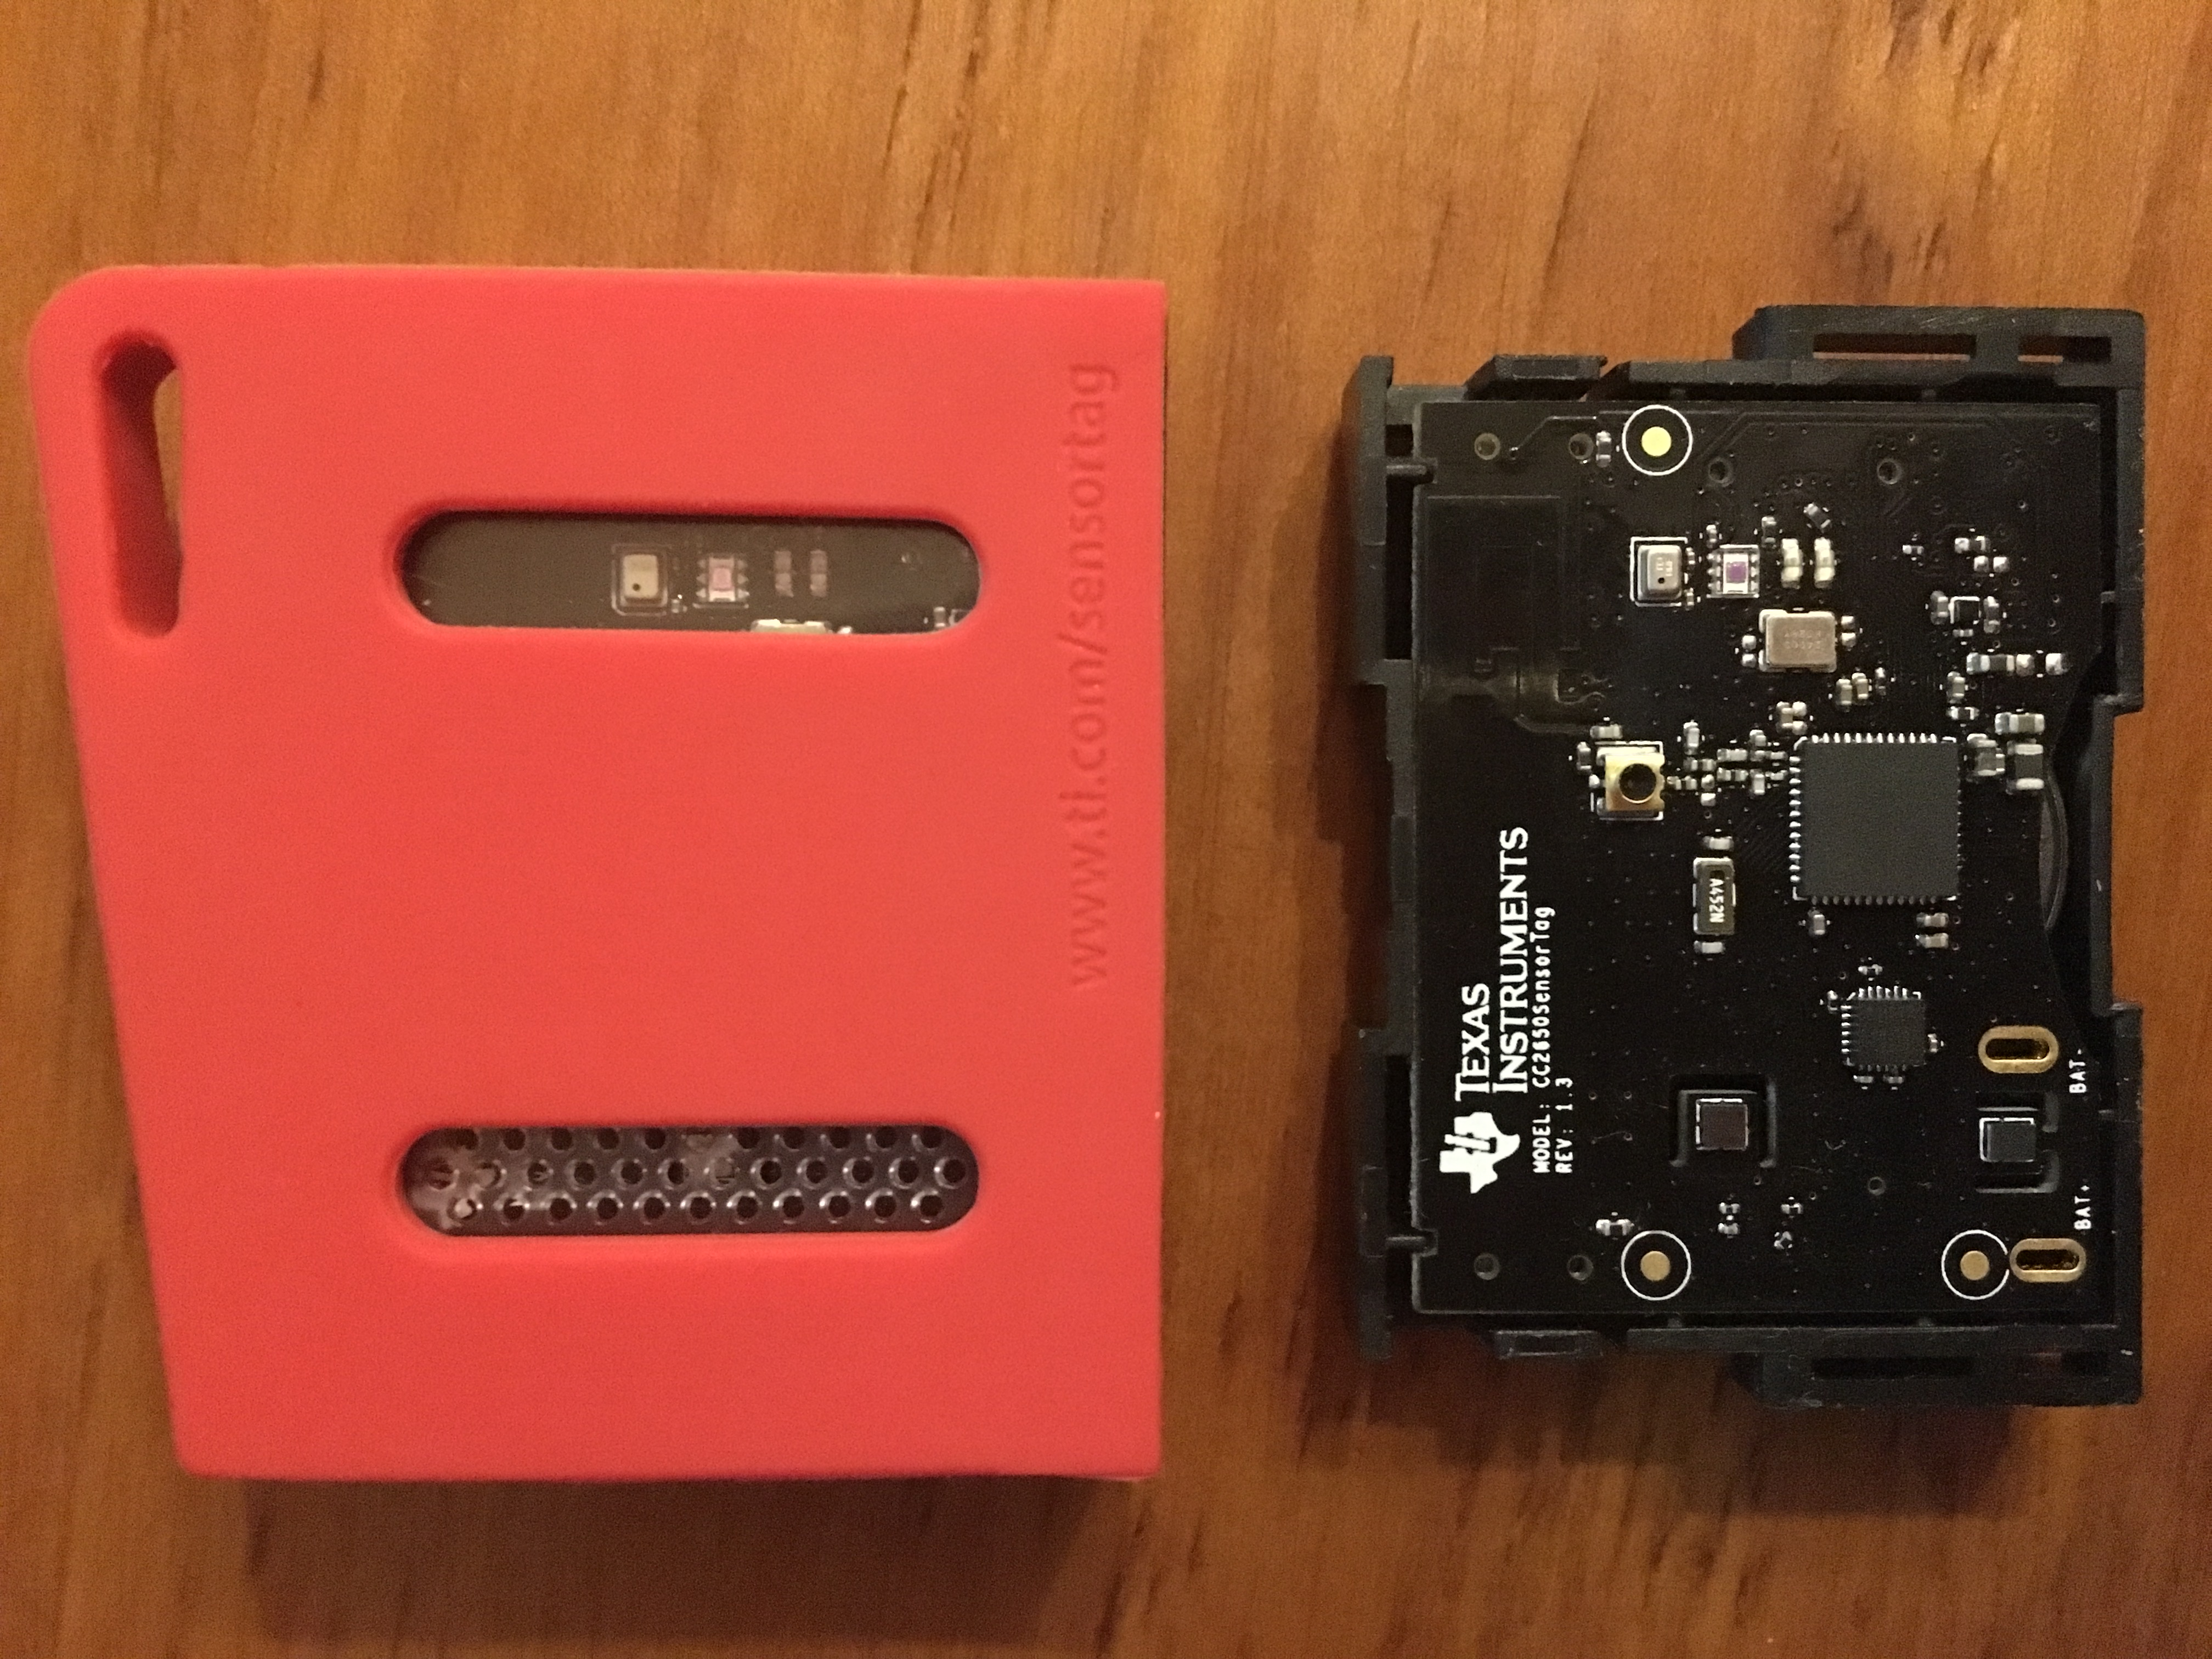
\includegraphics[width=0.5\linewidth]{4.Chapter/beacon.jpg}  
\caption[TI cc2650stk sensortag]{TI cc2650stk sensortag}  
\label{fig:beacon}  
\end{figure}  
 
 
The initial idea was to insert a new service into the already existing profile making use of the generic files provided by Texas.   
In order to implement the service, a characteristic containing the device's server IP and port was created and two random 128-bit universally unique identifier (UUID) were generated. When using UUIDs, the Bluetooth SIG defined several UUID, each associated with a certain service, such as heart rate or glucose services \cite{bleservices}. This situation makes it so that whenever one intends to implements a new service, one has to generate a random 128-bit UUID for his service and another one for each of required characteristics.  
Despite the efforts made, it wasn't possible to alter the existent profile by adding the new service neither by simply attempting to alter it by removing existent services. Due to the low amount of existent information on the technology an alternative was created. The solution found was to store the information into an already functioning service's characteristics as one was capable of altering those kind of parameters. The characteristics available to be used were only the ones from the device information service, a service defined by the Bluetooth sig, since the remaining services on the \ac{BLE} device were meant for reading values of from sensors. The chosen characteristic was the Manufacturer's name due to its low relevance and the fact that its UUID was known, while the remaining's weren't.  
  
 
 
  
In order to reduce the time complexity of the \ac{BLE} communication between the tags and the smartphone application, an attempt was made to reduce the number of connection to a minimum. With the objective of only attempting to communicate with tags that belong to the system while ignoring the remaining, a template name was given to each tag. By adding a common name component, such as \"BLE\_TAG\_SYSTEM\_\" and adding a second part that is device specific, one attempted to apply an initial filter on the nearby \ac{BLE} enabled devices.  
  
  
 
 
  
  
  
 
\section{Location service} 
\label{sec:LocService} 
 
 
The Smartphone application was developed for Android using the Android Studio IDE. The Application is divided in two primary functional blocks, the location service and maps service, as seen in figure \ref{fig:implementation}. 
 
 
The location service is implemented as if it was a Location provider, such as GPS. By implementing the whole process of obtaining a location inside a service, one extra level of abstraction is added to the application. As such, whenever the application is signaled to obtain the user's current location, a request is made to the associated location service and the application only needs to listen for the answer that will eventually arrive. 
 
 
 
 
 
 
The location service includes the first three steps presented in figure ~\ref{fig:MockProvider}, which will now be described individually. The initial step represents the gathering of information about user's surroundings. Upon receiving a location request, the service initiates a scan for nearby Bluetooth low energy beacon. This scanning puts the smartphone in a listening state for incoming \ac{BLE} advertisement packets. During this scanning period, each time a beacon is found, its name is analysed so that it can be compared with the used name template. Having passed through the first scanning, each beacon is registered for later usage. Once the scanning period is completed, the list of beacons is completed and forwarded for the next step. 
 
 
\begin{figure}[H] 
\centering 
\includegraphics[width=0.5\linewidth]{4.Chapter/RequestLocation.png} 
\caption[Application Workflow]{Application Workflow} 
\label{fig:MockProvider} 
\end{figure} 
 
 
The second step, in a summarised way, consists of communicating with each of the beacons, in order to obtain their location server's address and forwarding the list to it.  
 
 
Upon completing the first step, the location service communicates with each beacon individually. For each beacon the service will attempt to respond to the caught advertisement packet, so that a connection can be created. Once the connection is created, the service requests a list of the available services of the paired beacon. 
Once received, the list of services is searched for, in an attempt to find the system service's universally unique identifier (UUID). If the beacon doesn't have the UUID that the service is looking for, it can assume that the paired \ac{BLE} enabled beacon doesn't belong to the system, leading to the termination of the connection. If on the other hand, the UUID is present, a request for the service's characteristics is made.  
 
 
Upon obtaining the requested list, its content is examined with the objective of finding the UUID of the characteristic containing the address of the beacon's associated location server. This search has the objective of confirming that the service existent in this beacon is in fact the one that was implemented for the system, thus excluding the possibility of having a different service which happened to have the same UUID. For any service outside those that are documented in the Bluetooth Special Interest Group (SIG), who have a specific UUID attached to them, the UUID is generated randomly and as such there is a small chance of collision.  
 
 
Once the wanted characteristic is found, the service reads its value, i.e. the beacon's associated server address, and stores it in a list. This list will contain the servers of the beacons that were found, and for each address there will be a list corresponding to each beacon's ID and their corresponding received signal strength indicator (RSSI) values. In order to quicken the previously described process, the service could keep in cache the most recent contacted beacons. Upon obtaining a beacon's associated server address, this information could be stored in a cache. Therefore, before initiating any connection, the service can look up if the beacon's data is present on it. Whenever this search succeeds, no further work is necessary. This optimisation would largely reduce the required number of connections. 
 
 
When every beacon has been contacted, a voting system is actioned which will decide from the list of servers which one it will send the collected information to. The voting system uses an exponential function in order to attribute a weight to each server.  
The voting system was implemented with the intention of providing a thin security layer. Since every beacon has an associated weight, one expects that the sum of valid beacon's weight is capable of eliminating that of a nearby attacker. After calculating each server's weighted sum, the one with the highest is chosen. This server is selected as the one responsible for calculating the user's position.  
 
 
The third step involves a simple client/server tcp interaction. The service starts by formulating the message that it will later on send to the server. This message includes all pairs of beacon mac address and its associated RSSI value captured by the service on the first step. Once the message is constructed, the service attempts to create a connection with the location server. With the connection established, the message is forwarded to the server and the service is put onto a blocked state where it awaits for an answer. Upon arrival, the received answer is verified, its information processed and the connection is terminated. The information contained inside the received message is then transferred into a container capable of storing a geographic location, which is then passed onto the application. 
 
 
 
\section{Server} 
\label{sec:server} 
 
 
The web server was implement in Python 3.5 programming language. The program implements a tcp server capable of receiving multiple request at the same time. Each request starts with information sent from an application which includes an undefined amount of pairs of MAC address and associated RSSI value, each corresponding to a \ac{BLE} enabled device that was found and connected. Afterwards the list of pairs is filtered in order to remove any existent devices that are not present in the server's database of devices. Upon extracting all the foreign devices from the list, the locating algorithm is deployed. Once the location has been calculated, a message is sent back to the smartphone with its information.  
 
 
Each server has a database that includes only \ac{BLE} devices. An entry (description of a device) in this database is composed by the device's mac address, its longitude and latitude and its building, floor and room name. In addition to the database, a server can store additional location information such as the server's street, number, zip-code, city and country, allowing it to be transmitted to the client. This offers an additional level of location description to the user.  
 
\section{Application} 
\label{sec:app} 
 
 
The implemented android application is responsible for communication with both the location service, already presented in section \ref{sec:LocService}, and the maps service. 
 
 
When a user notifies the application that he wishes to start the system, the app starts a periodic operation that provides a location at the end of each iteration. At the beginning of each operation, the app requests the location service for a location. The expected answer contains a geographical location as well as additional  textual information. The data is then forwarded to the maps service. This action is the fourth and last from figure \ref{fig:MockProvider}. 
 
 
The maps service is implemented using the Google Maps Android API. Through the usage of Google Maps, it was possible to reduce the load on the application, since there was no need implement the maps server component. Since the indoor maps of the testing environment were already available, there was no need to upload addition maps onto google maps. Having passed the entire maps server component onto the already existent service, the complexity of the system was reduced. By making this development choice, the system as a whole became closer to the desired generic approach while making possible for seamless transition between indoor/outdoor maps. The only imposed restriction is related to the addiction of new indoor maps onto the google maps, which while possible and well documented, is dependent on a third party. As previously described on chapter \ref{cap:architecture}, upon deciding to use the google maps service as the maps server, the location description present in the location server had to be adjusted accordingly. The position description of each \ac{BLE} enable device contained in the database were updated, so that it would be compatible with the description type used by Google maps. This change involved describing each beacon by its latitude, longitude and floor level. 
 
 
The Fourth step occurs when the application receives a location from the request made onto the location provider. With the device's location known, a marker is placed on the map with the obtain coordinates (longitude, latitude), the camera is centralised on the position while displaying the indoor level map. The menu visible on figure ~\ref{fig:AppMenu} is updated with the information that is bundled with the received location. In order to show the correct level on a multi level building, the "floor" information present in the menu is used. The Google API is capable of providing a list of the levels of the building that is currently being focused by the map's camera. Since the location's associated floor is know, the floor can be selected from the list and the view updated. 
 
 
The pop-up menu was implemented to demonstrate the capacity of providing additional information associated with each location. While the current implementation displays the location's geo-location taxonomy, the architecture is capable of support other types of additional information, such as hyperlink or information on nearby events.   
 
 
The final state of the implemented system can be visualised in figure ~\ref{fig:AppFocus} and figure ~\ref{fig:AppMenu}. The first figure displays the applications main screen, where the google maps view is located. In this example: 
\begin{itemize} 
\item The user's location inside the building is represented by the red marker; 
\item The building where the user is located is focused. Upon focusing on a building, google maps provides a level selector. Through it, it's possible to select the building floor that is to be displayed; 
\item The building floor where the user is located is selected. This action updates the view with the selected floor and highlights it (floor 0) on the provided menu. 
\end{itemize} 
Figure \ref{fig:AppMenu} displays the menu containing the geo-location taxonomy. 
 
 
\begin{figure} 
\centering 
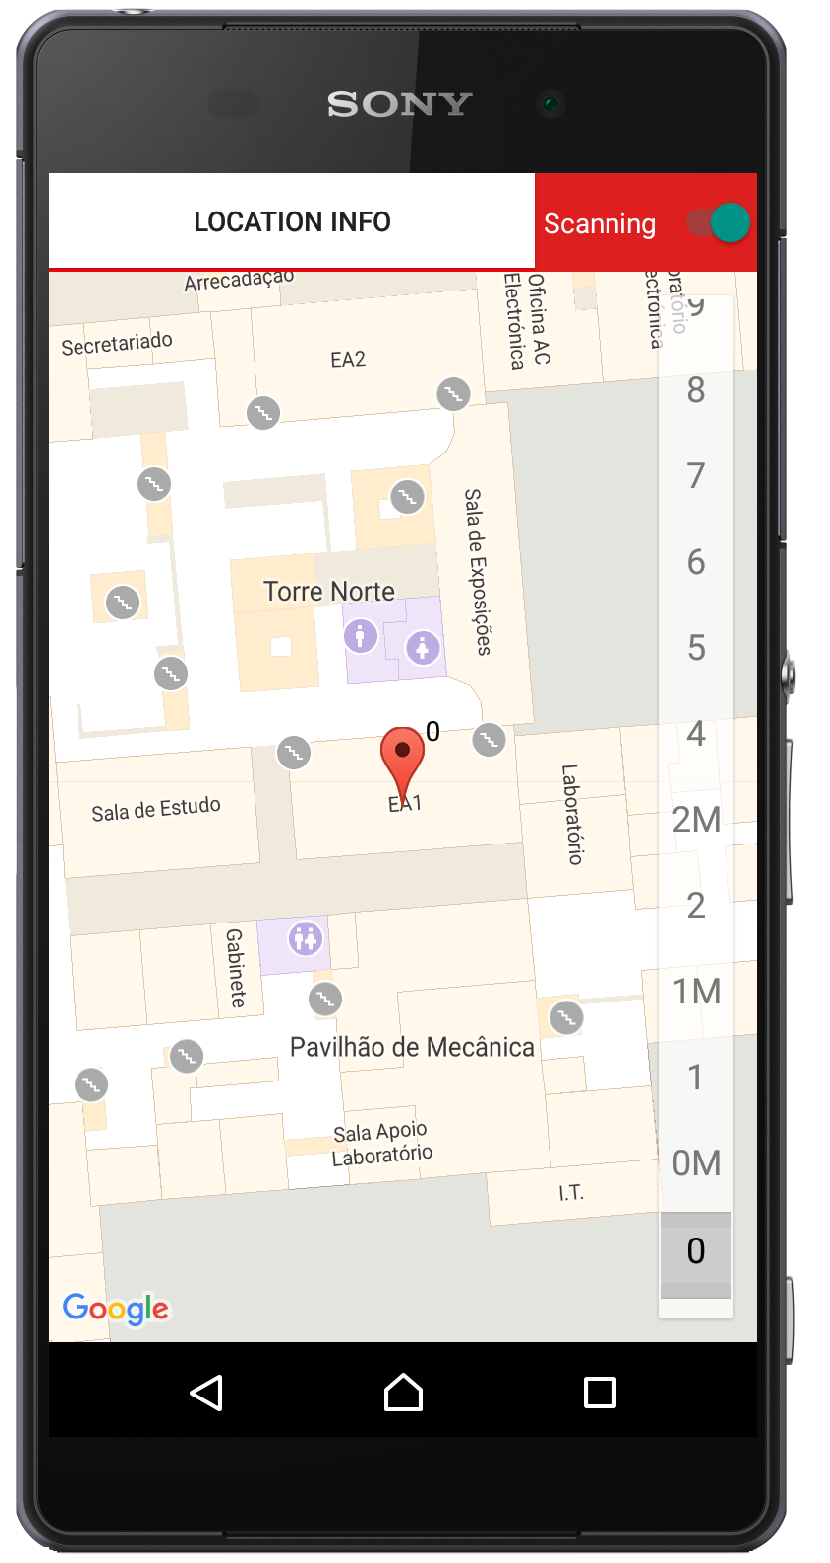
\includegraphics[width=0.5\linewidth]{4.Chapter/app_focused.png} 
\caption[Application screen showing a focused location on a room]{Application screen showing a focused location on a room} 
\label{fig:AppFocus} 
\end{figure} 
 
 
\begin{figure} 
\centering 
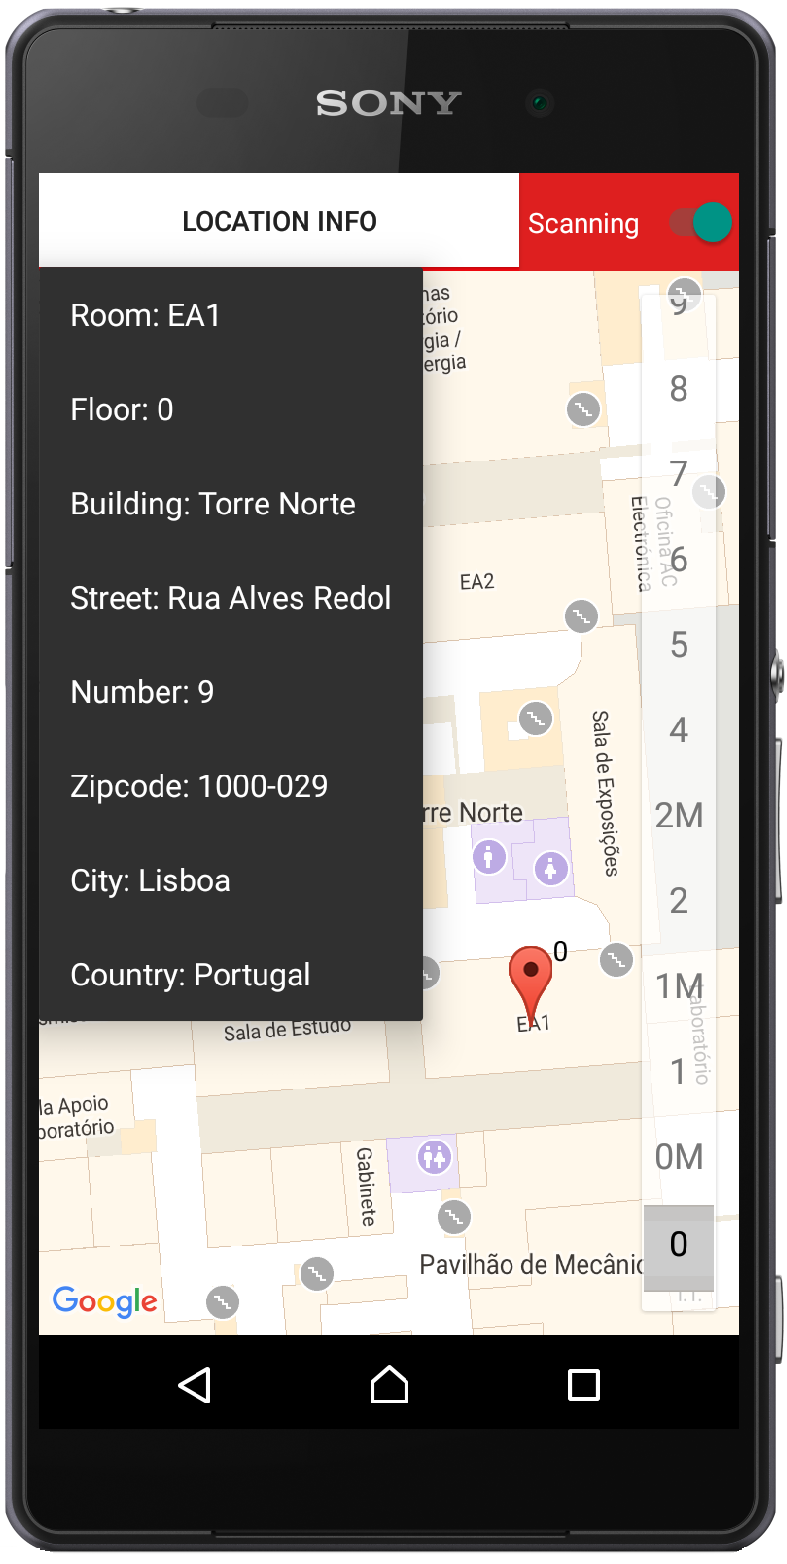
\includegraphics[width=0.5\linewidth]{4.Chapter/app_focused_menu.png} 
\caption[Application screen showing additional information of location]{Application screen showing additional information of location} 
\label{fig:AppMenu} 
\end{figure} 
 
 
 

\cleardoublepage
